\subsection{Advanced Evolution of Massive Stars}\label{sec:AdvancedEvolution}

After evolution to the main sequence, massive stars of initial mass $\gls{InitialMass} \gtrsim 8M_{\odot}$ build a C-O core of mass $\gls{CoreMass} \gtrsim 1.06M_{\odot}$ via He-burning to begin $^{12}$C-burning, producing isotopes such as $^{20}$Ne and $^{24}$Mg.

This moves to burning in a shell as Ne-burning begins in a convective core, forming $^{16}$O via photo-disintegration and alpha-capture (for stars $\gls{InitialMass} \gtrsim 11M_{\odot}$).
Likewise, this then moves into a shell before O-burning takes place via the $^{16}$O$+^{16}$O reaction to form $^{28}$Si and $^{32}$S within a convective core. 

Si-burning begins soon after O-burning moves to a shell, tending towards a final core composition of $^{56}$Fe and $^{52}$Cr, forming a core primarily of $^{56}$Fe before core collapse. 

As time progresses, evolutionary timescales become shorter, from $\sim 10^{3}\mathrm{yr}$ for $^{12}$C-burning to $\sim 1\mathrm{yr}$ for $^{16}$O-burning and only $\sim 10^{-2}\mathrm{yr}$ for $^{28}$Si-burning, sped up by neutrino emission increasing the rate of core contraction, thereby increasing temperatures between burns. This is reflected in both the ratio of energy generation to energy radiation (via neutrinos; $\gls{eta}$) and the increase in central density ($\gls{rhoc}$) per unit core temperature ($\gls{Tc}$) over time.

Notably, this relation deviates from almost constant proportionality before He-burning, to one with patterns characteristic of each burning stage, deviating from the trend due to the interplay between neutrino loss and temperature increase (\citealp{Polls11}; see Figure \ref{fig:TcRc_Compare}). 

\begin{figure}[H]
\begin{center}
    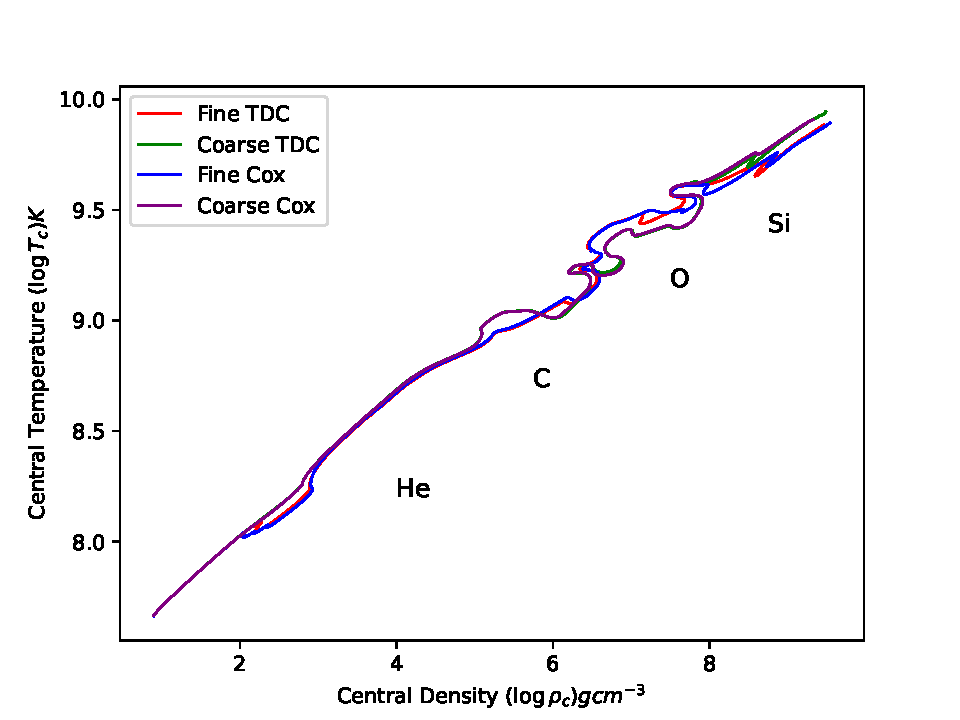
\includegraphics[width=0.9\linewidth]{TcRc_Compare}
    \caption{Graph of central temperature (\gls{Tc}) against central density (\gls{rhoc}), plotted from $35\%$ H in the core for four models varying by timestepping and mixing theory. Locations of burning stages are labelled (label locations based on \citealp{Maeder09}).}
    \label{fig:TcRc_Compare}
\end{center}
\end{figure}

Kippenhahn diagrams, such as in Figure \ref{fig:KHD_Compare_Metal} further aid analysis, showing the evolution of convective burning shells in terms of size (e.g. radius), convection (e.g. Mach number) and time to evolve. 

%\begin{figure*}[t]
\begin{center}
    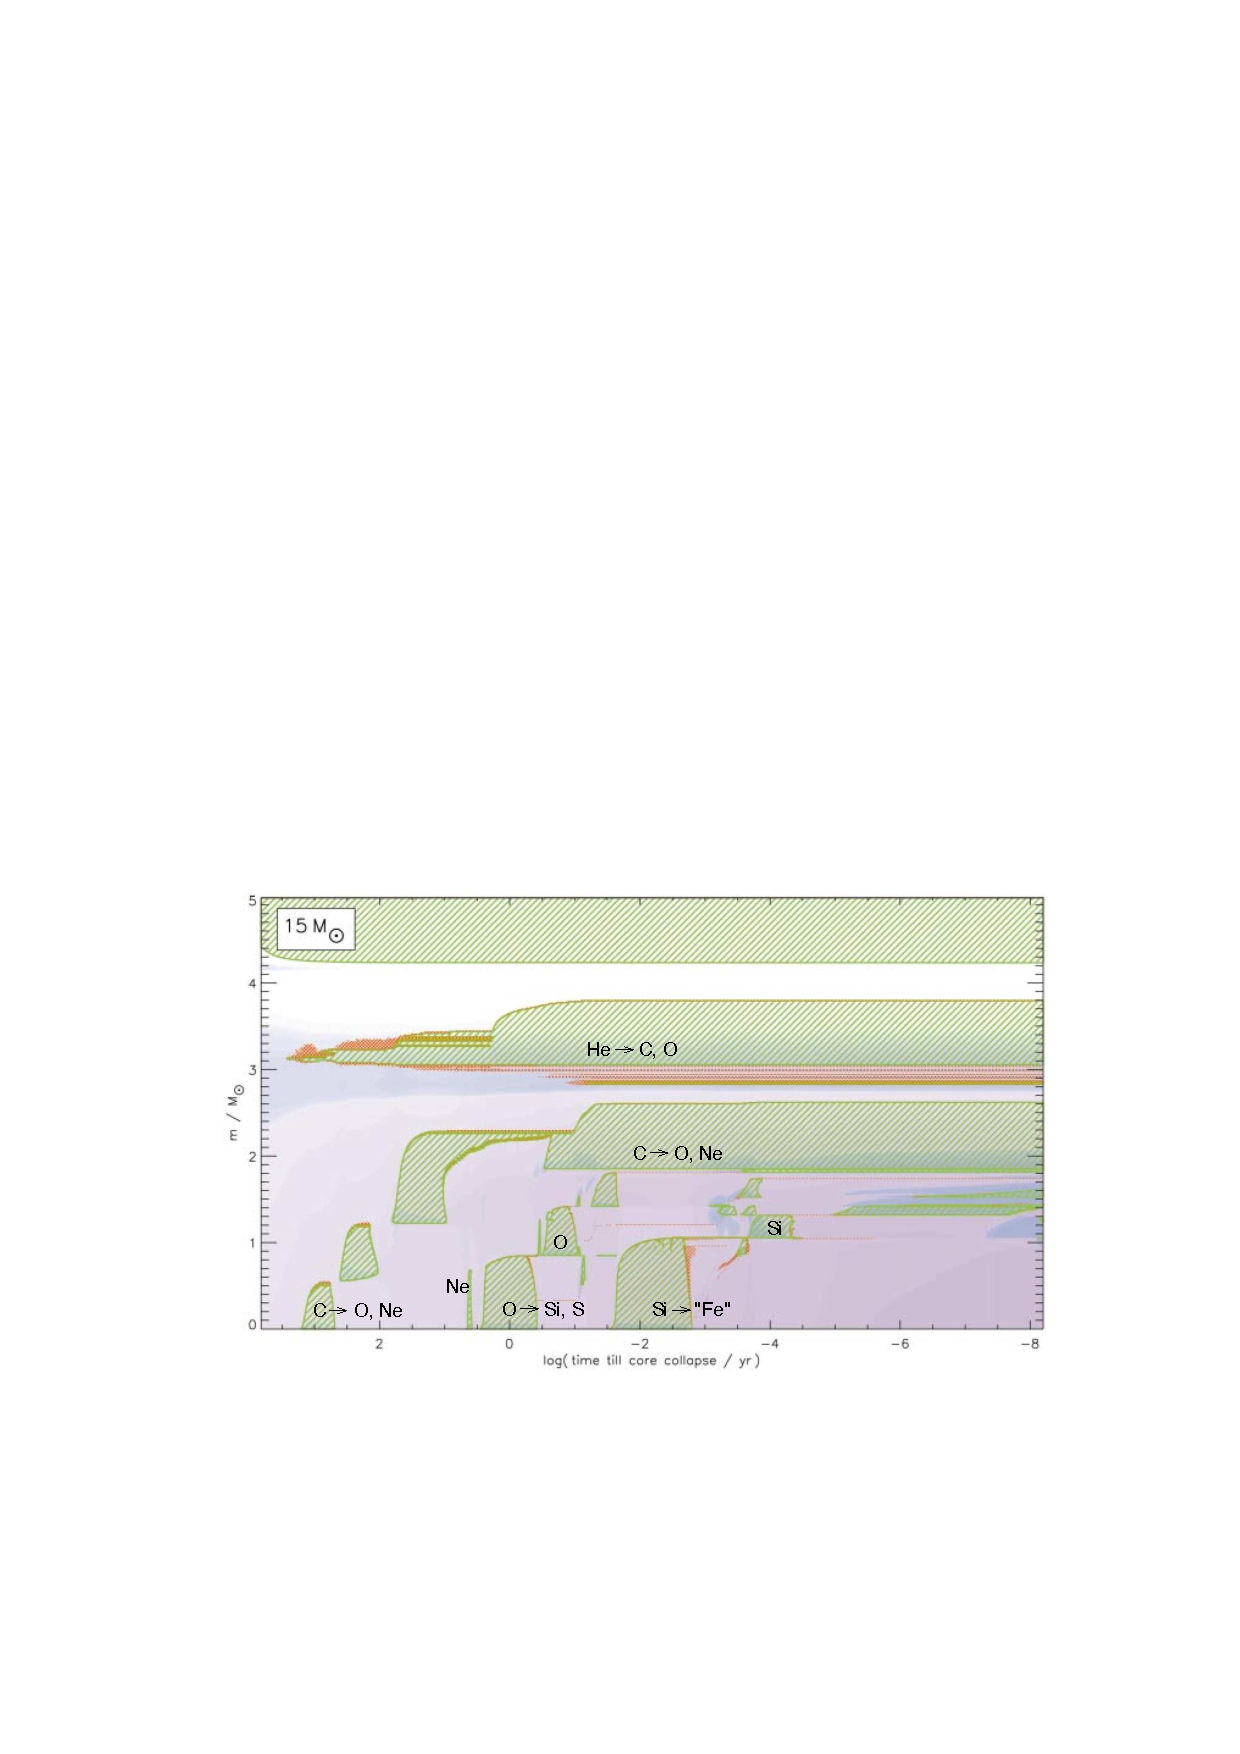
\includegraphics[width=0.8\linewidth]{Pols11_KHD}
    \caption{Kippenhahn diagram of mass by time until core collapse. The main burning stages are annotated (Figure from \citealp{Polls11}).}
    \label{fig:Polls11}
\end{center}
\end{figure*}
\begin{figure*}[t]
\begin{center}
    \includegraphics[width=0.7\linewidth]{Figures/KHD_Compare_Metal.pdf}
    \caption{Kippenhahn diagrams of radius (logarithmic) by time until core collapse, comparing a \gls{LowMetal} (lower) and \gls{SolarMetal} (upper) run using \gls{MLT} and short timestepping. Colour pertains to Mach number and label locations are based off of \citealp{Polls11}.}
    \label{fig:KHD_Compare_Metal}
\end{center}
\end{figure*}

Importantly, because the time between the onset of C-burning and core collapse is shorter than the dynamical timescale, $\gls{DynamicTimescale}$, there is insufficient time for effects experienced at or near the core (such as expansions) to have surface expressions (through changes in luminosity, \gls{lum}, or radius). \glspl{HRD}, such as in Figure \ref{fig:HDR_Compare}, exemplify this, with the majority of change in \gls{lum} and surface temperature, \gls{Teff}, occurring before C-burning commences.  

\begin{figure}[H]
\begin{center}
    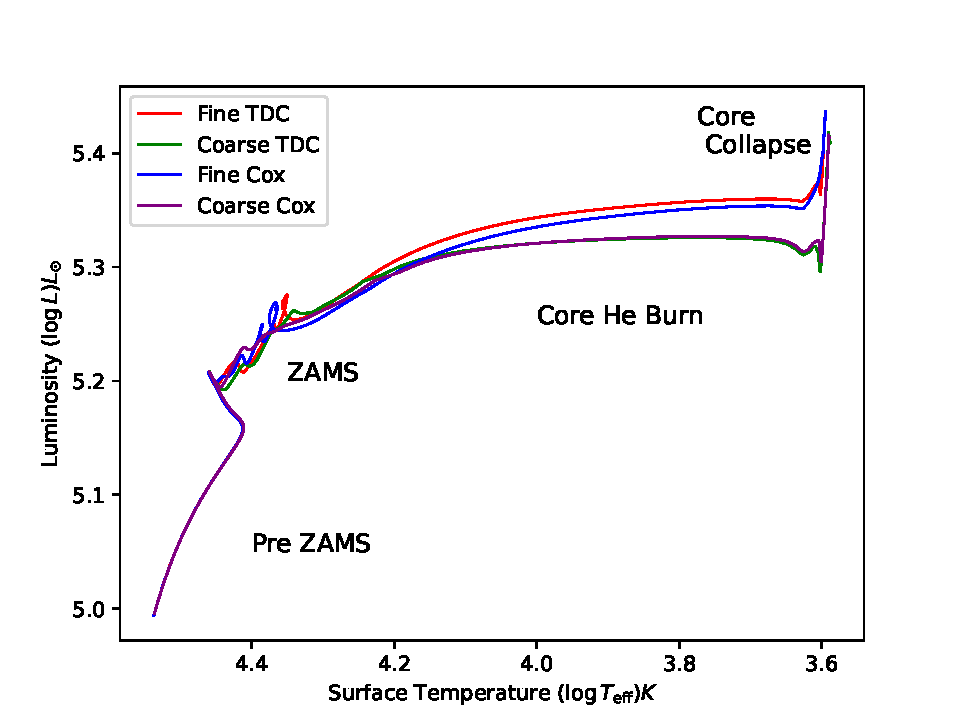
\includegraphics[width=0.9\linewidth]{Figures/HDR_Compare.pdf}
    \caption{\gls{HRD} showing change in luminosity by surface temperature of four models from H-burning at $35\%$ core He, varying only by mixing theory and resolution (Fine = high resolution, Coarse = test run resolution). Important stages are labelled (where ZAMS = zero age main sequence; label location after \citealp{Maeder09}).}
    \label{fig:HDR_Compare}
\end{center}
\end{figure}

%mention the theory behind the importance of studying convection

%{\tt MESA} also accounts for stellar wind using the scheme devised by \citet{deJager88}: an effect where photon momentum is efficiently transferred to outer envelope layers at $\gls{InitialMass} \gtrsim 15M_{\odot}$.

%reference de Jager? - https://ui.adsabs.harvard.edu/abs/1988A%26AS...72..259D/abstract